%%%%%%%%%%%%%%%%%%%%%%%%%%%%%%%%%%%%%%%%%%%%%%%%%%%%%%%%%%%%%%%%%%%%%%%%%%%%%%%
%                       CARREGA DE LA CLASSE DE DOCUMENT                      %
%                                                                             %
% Les opcions admissibles son:                                                %
%      12pt / 11pt            (cos dels tipus de lletra; no feu servir 10pt)  %
%                                                                             %
% catalan/spanish/english     (llengua principal del treball)                 %
%                                                                             %
% french/italian/german...    (si necessiteu fer servir alguna altra llengua) %
%                                                                             %
% listoffigures               (El document inclou un Index de figures)        %
% listoftables                (El document inclou un Index de taules)         %
% listofquadres               (El document inclou un Index de quadres)        %
% listofalgorithms            (El document inclou un Index d'algorismes)      %
%                                                                             %
%%%%%%%%%%%%%%%%%%%%%%%%%%%%%%%%%%%%%%%%%%%%%%%%%%%%%%%%%%%%%%%%%%%%%%%%%%%%%%%

\newcommand{\relativepath}{"style"}
\documentclass[11pt,spanish,listoffigures,listoftables]{\relativepath/tfgetsinf}

%%%%%%%%%%%%%%%%%%%%%%%%%%%%%%%%%%%%%%%%%%%%%%%%%%%%%%%%%%%%%%%%%%%%%%%%%%%%%%%
%                     CODIFICACIO DEL FITXER FONT                             %
%                                                                             %
%    windows fa servir normalment 'ansinew'                                   %
%    amb linux es possible que siga 'latin1' o 'latin9'                       %
%    Pero el mes recomanable es fer servir utf8 (unicode 8)                   %
%                                          (si el vostre editor ho permet)    %
%%%%%%%%%%%%%%%%%%%%%%%%%%%%%%%%%%%%%%%%%%%%%%%%%%%%%%%%%%%%%%%%%%%%%%%%%%%%%%%

\usepackage[utf8]{inputenc}

%%%%%%%%%%%%%%%%%%%%%%%%%%%%%%%%%%%%%%%%%%%%%%%%%%%%%%%%%%%%%%%%%%%%%%%%%%%%%%%
%                        ALTRES PAQUETS I DEFINICIONS                         %
%                                                                             %
% Carregueu aci els paquets que necessiteu i declareu les comandes i entorns  %
%                                          (aquesta seccio pot ser buida)     %
%%%%%%%%%%%%%%%%%%%%%%%%%%%%%%%%%%%%%%%%%%%%%%%%%%%%%%%%%%%%%%%%%%%%%%%%%%%%%%%

\usepackage{graphicx}
\usepackage{wrapfig}

%%%%%%%%%%%%%%%%%%%%%%%%%%%%%%%%%%%%%%%%%%%%%%%%%%%%%%%%%%%%%%%%%%%%%%%%%%%%%%%
%                        DADES DEL TREBALL                                    %
%                                                                             %
% titol, alumne, tutor i curs academic                                        %
%%%%%%%%%%%%%%%%%%%%%%%%%%%%%%%%%%%%%%%%%%%%%%%%%%%%%%%%%%%%%%%%%%%%%%%%%%%%%%%

\title{Refactorización de una infraestructura de bucles MAPE-K como microservicios}
\author{Adriano Vega Llobell}
\tutor{Joan Josep Fons Cors}
\curs{2021-2022}

%%%%%%%%%%%%%%%%%%%%%%%%%%%%%%%%%%%%%%%%%%%%%%%%%%%%%%%%%%%%%%%%%%%%%%%%%%%%%%%
%                     PARAULES CLAU/PALABRAS CLAVE/KEY WORDS                  %
%                                                                             %
% Independentment de la llengua del treball, s'hi han d'incloure              %
% les paraules clau i el resum en els tres idiomes                            %
%%%%%%%%%%%%%%%%%%%%%%%%%%%%%%%%%%%%%%%%%%%%%%%%%%%%%%%%%%%%%%%%%%%%%%%%%%%%%%%

\keywords{????, ?????????, ????, ?????????????????} % Paraules clau
         {?????, ???, ???????????????}              % Palabras clave
         {?????, ????? ?????, ?????????????}        % Key words

%%%%%%%%%%%%%%%%%%%%%%%%%%%%%%%%%%%%%%%%%%%%%%%%%%%%%%%%%%%%%%%%%%%%%%%%%%%%%%%
%                              INICI DEL DOCUMENT                             %
%%%%%%%%%%%%%%%%%%%%%%%%%%%%%%%%%%%%%%%%%%%%%%%%%%%%%%%%%%%%%%%%%%%%%%%%%%%%%%%
\begin{document}

\bibliographystyle{ieeetr}

%%%%%%%%%%%%%%%%%%%%%%%%%%%%%%%%%%%%%%%%%%%%%%%%%%%%%%%%%%%%%%%%%%%%%%%%%%%%%%%
%              RESUMS DEL TFG EN VALENCIA, CASTELLA I ANGLES                  %
%%%%%%%%%%%%%%%%%%%%%%%%%%%%%%%%%%%%%%%%%%%%%%%%%%%%%%%%%%%%%%%%%%%%%%%%%%%%%%%

\begin{abstract}
????
\end{abstract}
\begin{abstract}[spanish]
????
\end{abstract}
\begin{abstract}[english]
????
\end{abstract}

%%%%%%%%%%%%%%%%%%%%%%%%%%%%%%%%%%%%%%%%%%%%%%%%%%%%%%%%%%%%%%%%%%%%%%%%%%%%%%%
%                              CONTINGUT DEL TREBALL                          %
%%%%%%%%%%%%%%%%%%%%%%%%%%%%%%%%%%%%%%%%%%%%%%%%%%%%%%%%%%%%%%%%%%%%%%%%%%%%%%%

\mainmatter

%%%%%%%%%%%%%%%%%%%%%%%%%%%%%%%%%%%%%%%%%%%%%%%%%%%%%%%%%%%%%%%%%%%%%%%%%%%%%%%
%                         CAPITOLS (tants com calga)                          %
%%%%%%%%%%%%%%%%%%%%%%%%%%%%%%%%%%%%%%%%%%%%%%%%%%%%%%%%%%%%%%%%%%%%%%%%%%%%%%%

%%%%%%%%%%%%%%%%%%%%%%%%%%%%%%%%%%%%%%%%%%%%%%%%%%%%%%%%%%%%%%%%%%%%%%%%%%%%%%%
%                                  INTRODUCCIO                                %
%%%%%%%%%%%%%%%%%%%%%%%%%%%%%%%%%%%%%%%%%%%%%%%%%%%%%%%%%%%%%%%%%%%%%%%%%%%%%%%

\chapter{Introducción}
\label{chap:introduccion}

%% TODO: Descripción de sistemas autónomos.

En este trabajo se quiere abordar la división de un servicio monolítico y adaptarlo para su funcionamiento en entornos en la nube. Para ello, se quiere extraer su funcionalidad en distintos microservicios. Es decir, se quiere \textbf{cambiar la topología} de la solución. Se trata de un cambio importante en la arquitectura de la solución.

%% TODO: ¿Multi-tennant? ¿Solución inicial muy acoplada y ad-hoc a una solución concreta? Se quiere independizar del programa.

En concreto, se trata de un servicio que implementa un bucle de control MAPE-K \cite{ArchitecturalBlueprintAutonomic2006, fonsServiciosAdaptivereadyPara2021}, una para la implementación de sistemas autónomos propuesta inicialmente por IBM. El bucle se encarga de gestionar un \textbf{recurso manejado} en base a unas \textbf{políticas} definidas por el administrador del sistema. Las políticas

En la figura \ref{fig:bucle-mapek} tenemos una representación de la arquitectura del bucle.

\begin{figure}[h]
  \centering
  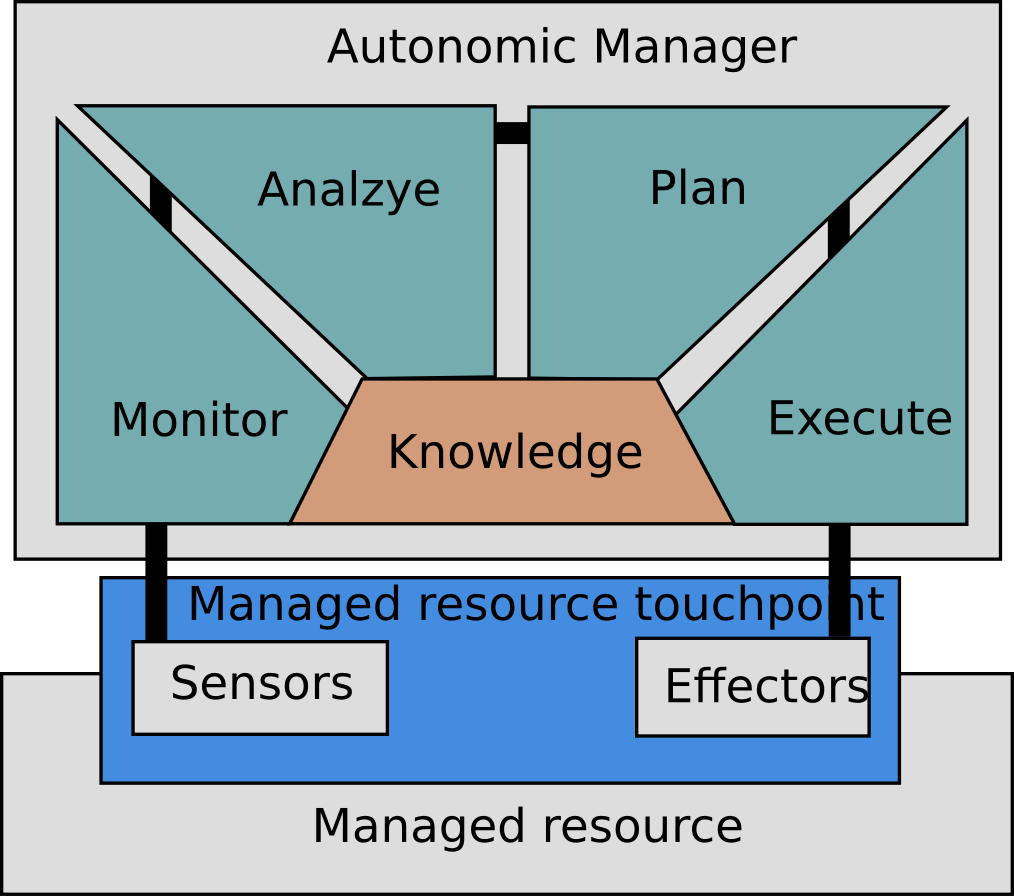
\includegraphics{01_introduccion/images/bucle-mape-k.png}
  \caption[Representación del Bucle MAPE-K]{Representación del Bucle MAPE-K.\footnotemark}
  \label{fig:bucle-mapek}
\end{figure}

% TODO: Cambiar por otra imagen sin typos.
\footnotetext{Obtenido de: \url{https://wwwvs.cs.hs-rm.de/vs-wiki/index.php/(WS12-01)_Cloud/Dokumentation}}


El recurso manejado puede ser un sistema \textit{hardware} o \textit{software} cualquiera. El único requisito es que debe implementar los \textbf{\textit{touchpoints}} (\textcolor{red}{puntos de contacto?}): interfaces que permiten al bucle de control obtener información del estado del sistema y cambiar su configuración en base a las políticas. Hay dos tipos de \textit{touchpoints}: \textbf{sondas} y \textbf{efectores}.

Las sondas reportan al bucle información del estado del sistema. Puede ser cualquier tipo de métrica que queramos controlar. Por ejemplo, \textit{health checks}, información de salud de la aplicación; propiedades del sistema que queramos controlar.

Por otro lado, los efectores, nos ayudan a modificar el estado del sistema manejado. Pueden ser ficheros de configuración, comandos, etc.

En la figura \ref{fig:bucle-mapek} podemos apreciar que el bucle puede dividirse en 5 componentes distintos: \cite{ArchitecturalBlueprintAutonomic2006}

\begin{itemize}
  \item \textbf{Base de conocimiento}: almacena el conocimiento relevante para la operación del bucle de control. Es tanto información del sistema como información del entorno de operación. Cada una de las claves almacenadas se conoce también como \textbf{propiedad de adaptación}.

  El conocimiento se comparte entre todos los componentes del bucle de control.

  \item \textbf{Monitor}: Recibe mediciones de las sondas del recurso manejado. Se encarga de recoger, agregar y filtrar estas mediciones para determinar si ha ocurrido un evento relevante que deba ser reportado. Por ejemplo, si la temperatura de una habitación supera un umbral definido por el usuario.

  \item \textbf{Analizador}: Conjunto de \textbf{reglas de adaptación} que se suscriben a las propiedades de adaptación. Están compuestas una condición y una acción. Cada vez que cambie alguna de las propiedades de las que dependen, se evalua su condición. Si esta se cumple, se ejecuta la acción asociada, que suele ser una propuesta de cambio en la configuración del sistema.

  \item \textbf{Planificador}: Si se ha llegado a ejecutar alguna regla de apdatación, el planificador recoge sus propuestas de cambio y determina las acciones necesarias para cumplir el objetivo.

  \item \textbf{Ejecutor}: Recibe
\end{itemize}

La idea es separar cada una de sus etapas en microservicios individuales. De esta forma, podemos desarrollarlas de forma independiente entre ellas, replicarlas para mejorar su escalabilidad, o sustituirlas por implementaciones distintas, etc.

Para desarrollar el trabajo, propusimos el siguiente plan:
\begin{itemize}
  \item Cada etapa del bucle será un microservicio distinto. Extraeremos cuatro microservicios distintos: Planificador, Analizador,
\end{itemize}

Por tanto, los conectores elegidos para comunicar los microservicios han sido más centrados en comunicar con las APIs públicas que expone cada uno.

\section{Motivación}

????? ????????????? ????????????? ????????????? ????????????? ?????????????

\section{Objetivos}

????? ????????????? ????????????? ????????????? ????????????? ?????????????

\section{Estructura de la memoria}

????? ????????????? ????????????? ????????????? ????????????? ?????????????

%\section{Notes bibliografiques} %%%%% Opcional

%????? ????????????? ????????????? ????????????? ????????????? ?????????????


\chapter{Arquitecturas de \textit{software}}

Según \cite{taylorSoftwareArchitectureFoundations2009}, la {\bf arquitectura de un sistema \textit{software}} es el conjunto de todas las decisiones de diseño principales que se toman durante la vida del sistema, aquellas que sientan las bases del desarrollo. \textcolor{red}{Se podría establecer un simil con los planos de construcción de un edificio.} Estas decisiones no solo se toman durante su concepción, si no también durante su desarrollo y posterior evolución.

La arquitectura afecta a todos los apartados del sistema: su estructura, funcionalidad, la implementación\dots Por ejemplo, una decisión de diseño principal que se suele tomar en las fases tempranas del desarrollo es la elección de la topología para la solución. Optar por desarrollar un servicio monolítico o una arquitectura basada en microservicios va a condicionar prácticamente todo el desarrollo. Desde el diseño, la implementación, el testeo, y sobre todo, el despliegue y operación. \textcolor{red}{Por tanto, es vital dedicar tiempo para definir la arquitectura en base a las necesidades de nuestro sistema.}

\section{Decisiones principales de diseño}

Las decisiones principales de diseño normalmente se resumen en comparativas entre distintas alternativas, cada una de ellas con sus ventajas e inconvenientes. Con el paso del tiempo, y con el avance del desarrollo, estas elecciones comienzan a asentarse, y se vuelven más dificiles de cambiar o rectificar.

Pueden tomarse en base a distintos criterios. Entre ellos podemos destacar: [Citation needed]

    \begin{itemize}
        \item \textbf{Requisitos del sistema:} a partir del dominio y las necesidades de nuestros usuarios, podemos deducir: la funcionalidad a implementar, las restricciones que debemos respetar y otras propiedades que debe poseer el sistema.

        \item \textbf{Arquitectura actual:} las decisiones tomadas previamente también condicionan las elecciones que se tomen más adelante. Cuanto más avanza el desarrollo, más se asientan las decisiones previas, y más dificil es rectificarlas.

        \item \textbf{Experiencia previa:} del desarrollo de este u otros sistemas. Podemos obtener métricas del funcionamiento y uso de nuestro sistema para informar decisiones futuras. \textcolor{red}{[Cita devops]}
    \end{itemize}

\section{Componentes de una arquitectura}

Según el estándar IEEE 42010-2011 \cite{ieeeStandard420102011Systems2011}, la arquitectura de un sistema es "\textit{un conjunto de conceptos o propiedades fundamentales, personificados por sus elementos, sus relaciones, y los principios que guían su diseño y evolución}". Nos provee de un marco de referencia común, de decisiones que nos nos provee con un vocabulario común, que nos permite describir sistemas

Por tanto, podemos describirla usando tres conceptos: \cite{perryFoundationsStudySoftware1992}

    \begin{itemize}
        \item \textbf{Componentes:} Son las piezas fundamentales que componen el sistema. Implementan la funcionalidad de la aplicación. Se utilizan para describir \textit{qué} partes conforman el sistema. Por ejemplo: un módulo, un servicio web...

        \item \textbf{Forma:} El conjunto de propiedades y relaciones entre los elementos o el entorno de operación. Describe \textit{cómo} está organizado el sistema. Por ejemplo: un servicio contacta con otro a través de una API.

        \item \textbf{Justificación:} Razonamiento o motivación de las decisiones que se han tomado. Responden al \textit{por qué} algo se hace de determinada forma. Normalmente no pueden deducirse a partir de los elementos y la forma, por lo que es necesario describirlos.

    \end{itemize}

\textcolor{red}{La arquitectura de un sistema puede contar con diferentes vistas, según aquel aspecto que deseemos resaltar. Por ejemplo, puede interesarnos más la interacción entre los componentes. O cosas por el estilo.}

Durante el diseño, para lidiar con la complejidad que pudiera alcanzar el sistema, solemos recurrir a descomponerlos usando diseños modulares: sistemas compuestos por unidades de funcionalidad que tienen una función específica. \cite{taylorSoftwareArchitectureFoundations2009} Estos elementos funcionales son los componentes. Dependiendo de las características de nuestro sistema, pueden tomar distintas formas: módulos dentro un mismo proceso, servicios distribuidos, etc.

Como hemos comentado antes, un sistema está conformado por \textbf{componentes} que implementan la funcionalidad de la aplicación. No suelen trabajar de forma aislada, si no que trabajan conjuntamente para realizar tareas más complejas. Por tanto, un aspecto clave es la integración y la interacción entre ellos. \cite{mehtaTaxonomySoftwareConnectors2000}

Para que dos o más componentes puedan interactuar, necesitamos definir un mecanismo de comunicación. Para ello, recurrimos a los \textbf{conectores}: se trata de elementos arquitectónicos que nos ayudan a diseñar y razonar sobre la comunicación entre componentes. Representan la transferencia de datos y de control entre componentes. En la figura \ref{fig:componentesEjemplo} mostramos una representación de la necesidad de comunicación entre dos componentes a través de un conector. No se ha especificado todavía ningún detalle sobre cómo se implementará. De esta forma, podemos estudiar la arquitectura y elegir los mecanismos adecuados para cada interacción del sistema. \cite{taylorSoftwareArchitectureFoundations2009}.

%% TODO: Los conectores son application-independent. No dependen de la funcionalidad de la aplicación.
%% TODO: Hablar de la cardinalidad de los conectores.

\begin{figure}[h!]
  \centering
  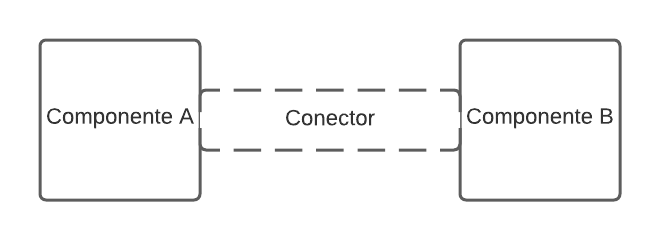
\includegraphics[scale=0.78]{02_arquitectura/images/conector}
  \caption{Ejemplo de comunicación de dos componentes a través de un conector.}
  \label{fig:componentesEjemplo}
\end{figure}

\textcolor{red}{A nivel de ¿diseño?}, los conectores están compuestos por uno o más \textbf{conductos} o canales de comunicación. A través de estos se lleva a cabo la comunicación entre los componentes. Hay una gran variedad de conductos posibles: comunicación interproceso, a través de la red, etc. Clasificamos los conectores según la complejidad de los canales que utilizan \cite{mehtaTaxonomySoftwareConnectors2000}:

\begin{itemize}
    \item \textbf{Conectores simples}: solo cuentan con un conducto, sin lógica asociada. Son conectores sencillos. Suelen estar ya implementados en los lenguajes de programación. Por ejemplo: una llamada a función en un programa o el sistema de entrada / salida de ficheros.

    \item \textbf{Conectores complejos}: cuentan con uno o más conductos. Se definen por composición a partir de múltiples conectores simples. Además, pueden contar con funcionalidad para manejar el flujo de datos y/o control. Suelen utilizarse importando \textit{frameworks} o librerias. Por ejemplo: un balanceador de carga que redirige peticiones a los nodos.
\end{itemize}

Por tanto, una vez hemos decidido que dos componentes deben comunicarse, es momento de evaluar cuál es el mecanismo de comunicación más adecuado. Para ello, podemos consultar la taxonomía de conectores de \cite{mehtaTaxonomySoftwareConnectors2000}. Basándonos en nuestros requisitos, la arquitectura ya definida, y los mecanismos de despliegue que queremos usar, elegimos el conector más adecuado.

\section{Arquitectura de la solución}

Como comentamos en el \autoref{chap:introduccion}: \nameref{chap:introduccion}, el objetivo del trabajo es adaptar un servicio monolítico para que funcione como un sistema distribuido basado en microservicios. Se trata de un cambio arquitectonico importante. Por ello, queremos diseñar una solución ingenieril teniendo en cuenta las particularidades del sistema.

Este servicio implementa un \textbf{bucle de control}, útil para dotar a un sistema con capacidades de computación autonoma. Especificamente, sigue la arquitectura del bucle MAPE-K\cite{ArchitecturalBlueprintAutonomic2006,fonsServiciosAdaptivereadyPara2021}, que mostramos en la figura \ref{fig:bucle-mapek2}. El objetivo de partida fue separar cada uno de los componentes del bucle en microservicios independientes.  \textcolor{red}{AÑADIR IMAGEN EJEMPLO DEL BUCLE DESCOMPUESTO EN MICROSERVICIOS. BUSCAR REFERENCIAS DE LIBROS SOBRE DIVIDIR MONOLITOS.}

\begin{figure}[h]
  \centering
  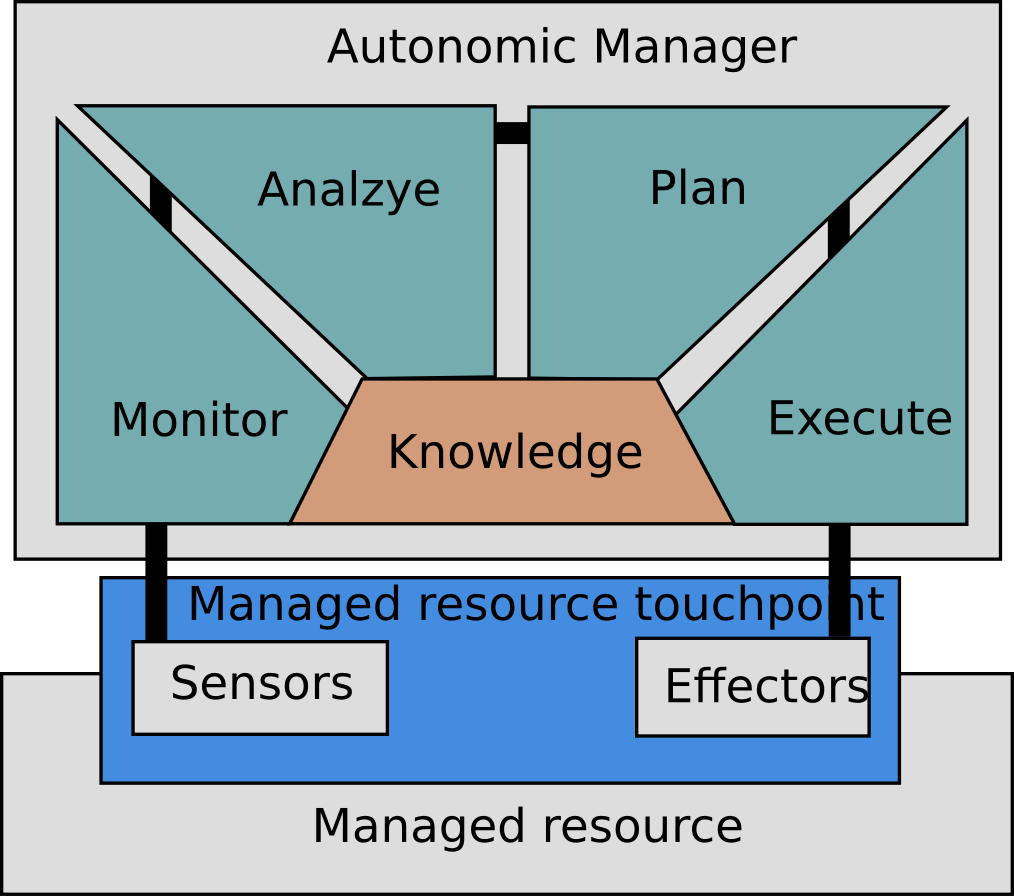
\includegraphics[scale=0.6]{01_introduccion/images/bucle-mape-k.png}
  \caption[Arquitectura de un Bucle MAPE-K.]{Arquitectura de un Bucle MAPE-K.\footnotemark}
  \label{fig:bucle-mapek2}
\end{figure}

% TODO: Cambiar por otra imagen sin typos.
\footnotetext{Obtenido de: \url{https://wwwvs.cs.hs-rm.de/vs-wiki/index.php/(WS12-01)_Cloud/Dokumentation}}

\textcolor{red}{Combinar con párrafo anterior: Actualmente, el sistema es un servicio monolitico que está muy acoplado a la solución. Queremos desacoplarlo para que pueda usarse la misma infraestructura para varios sistemas (\textit{multi-tennancy})}.

\subsection{Distribución de los componentes}

Por suerte, partimos de un sistema existente, con una arquitectura bien definida y documentada. Conociamos el rol de los componentes del servicio y sus requisitos. Asi que, el primer problema al que nos enfrentamos estaba relacionado con la distribución de los servicios. ¿Cómo definimos las fronteras entre cada uno de ellos?

Una vez determinadas las "fronteras" entre los microservicios, hemos definido los componentes de nuestro sistema. Asi que, el primer problema al que nos enfrentamos estaba relacionado con la comunicación: si separamos las distintas etapas del bucle en microservicios, ¿cómo hacemos para que se comuniquen? Hay que tener en cuenta que estos pueden estar desplegados y replicados en distintas máquinas.

Por la descripción de ambos componentes, vemos que existe una clara división de dominios y responsabilidades. Esto nos ayuda a determinar que ambos componentes pueden desplegarse por separado. \textcolor{red}{REFERENCIA 'Building Microservices' Sam Newman}

\textcolor{red}{TODO: Layered architecture. Dos capas: Distinguimos entre los microservicios clientes (monitores / sensores, reglas especifícas, etc) (círculo externo) y los microservicios de nuestro bucle MAPE-K (monitoring service, knowledge service...) (círculo interno). De esta forma podemos distinguir las responsabilidades de cada capa y como ocurre la comunicación entre ellas. Restringir la dirección de la comunicación por niveles. Comandos hacia arriba, notificaciones hacia abajo. Por ej: Podría ocurrir que cuando la información viene del dominio ''hacia dentro'', la comunicación sea a través de APIs REST y clientes autogenerados con OpenAPI. Pero, cuando la información fluye del bucle ''hacia fuera'', por ej del Analyser a las reglas, se hace mediante brokers de mensajería -> Menos acoplamiento.}

\textcolor{red}{AMPLIAR}

\begin{figure}[h]
  \centering
  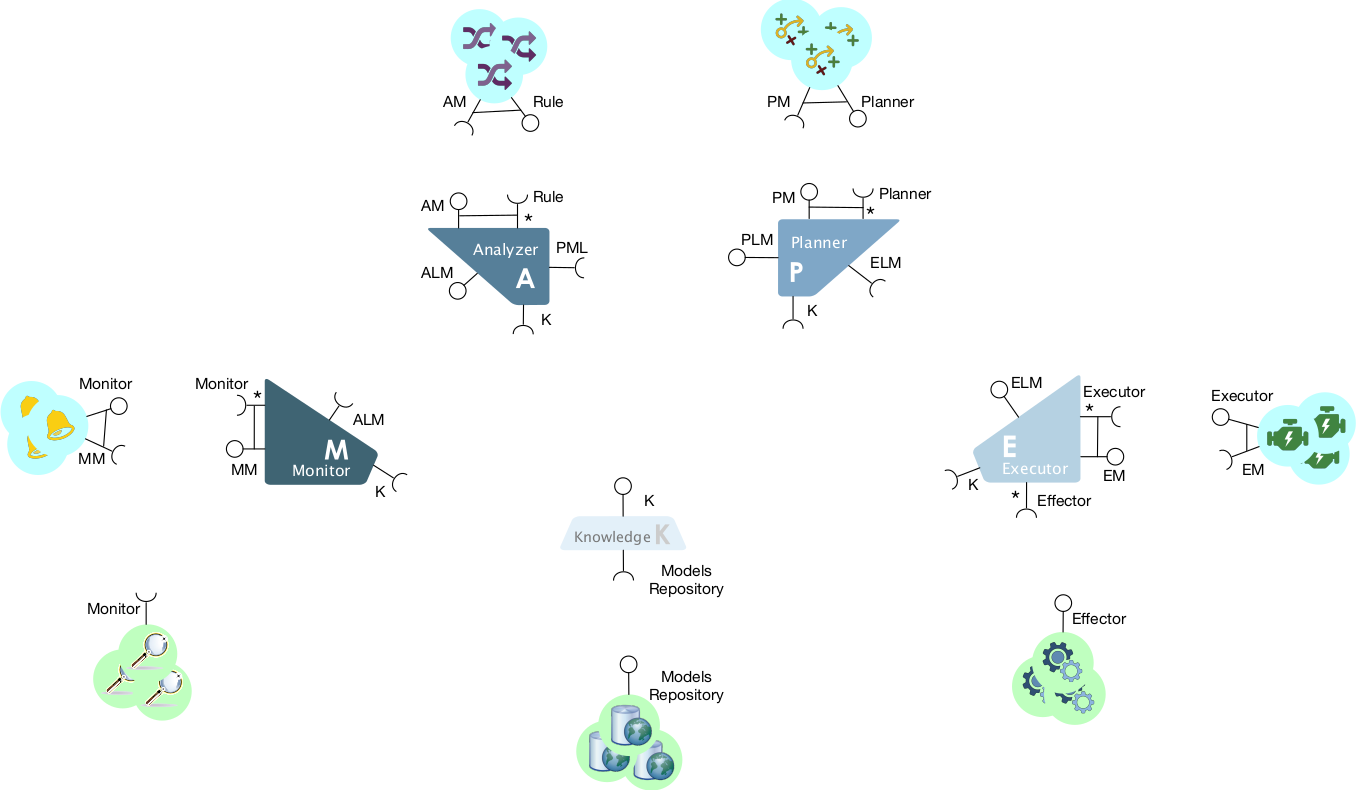
\includegraphics[scale=0.3]{02_arquitectura/images/mape-k-microservices}
  \caption{Diagrama con los componentes que forman nuestra arquitectura distribuida}
  \label{fig:mape-k-microservices}
\end{figure}

\subsection{Comunicación entre componentes}

Una vez determinadas las ''fronteras'' entre los microservicios, hemos definido los componentes de nuestro sistema. El siguiente problema al que nos enfrentamos fue la comunicación: si separamos las distintas etapas del bucle en microservicios, ¿cómo hacemos para que se comuniquen? Debemos tener en cuenta que estos pueden estar desplegados en máquinas distintas.

Comenzamos entonces la búsqueda de los conectores más apropiados para cada par de componentes. Seguimos la estrategia descrita en \cite{taylorSoftwareArchitectureFoundations2009} y consultando patrones de comunicación en sistemas distribuidos descritos en \cite{newmanBuildingMicroservicesDesigning2021}. \textcolor{red}{AMPLIAR} Comenzamos eligiendo qué dos componentes queremos conectar.

Tomemos por ejemplo la comunicación entre el servicio de monitorización (\textit{monitoring service}) y el servicio de conocimiento (\textit{knowledge service}). Recordemos que el servicio de conocimiento almacena todas las propiedades de adaptación. El resto de servicios necesitan consultar y actualizarlas durante su funcionamiento. En la figura \ref{fig:monitor-knowledge-initial} representamos inicialmente ambos componentes y un conector, sin especificar de qué tipo será.

\begin{figure}[h]
  \centering
  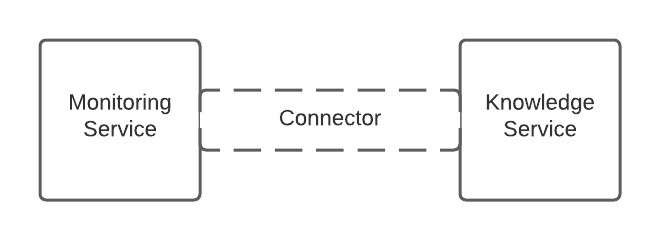
\includegraphics{02_arquitectura/images/Monitor-Knowledge-Initial-Connector}
  \caption{Boceto inicial: queremos conectar el servicio de monitorización con la base de conocimiento para poder leer propiedades de adaptación.}
  \label{fig:monitor-knowledge-initial}
\end{figure}

El siguiente paso es identificar qué interacciones debe existir entre ambos componentes. En este caso, el servicio de monitorización debe contactar con el servicio de conocimiento para leer y actualizar el valor de las propiedades. Por tanto, existen operaciones de lectura y escritura de los datos.

Ahora, debemos identificar qué \textbf{tipos de conector} serían adecuados para nuestros componentes. Sabiendo que hemos optado por una arquitectura distribuida, la elección se simplifica: los servicios pueden estar desplegados en máquinas distintas, por tanto el paso de mensajes será a través de la red.

Sabiendo esto, en lugar de recurrir a la taxonomía que lista \cite{mehtaTaxonomySoftwareConnectors2000}, optamos por consultar las estrategias de comunicación habituales para sistemas distribuidos descritas en \cite{newmanBuildingMicroservicesDesigning2021}. Se trata de cuatro mecanismos distintos: Invocación a métodos remotos (\textit{Remote Procedure Call}), APIs REST, consultas con GraphQL o \textit{brokers} de mensajería. Tuvimos que evaluarlos mediante un análisis de \textit{trade-offs} para determinar las ventajas y desventajas de cada uno.

\begin{itemize}
  \item \textbf{Invocación de métodos remotos} o (\textit{\textbf{Remote Procedure Call}}): Se trata de un paradigma de objetos distribuidos. \cite{taylorSoftwareArchitectureFoundations2009} Nuestro programa interactúa con objetos que se encuentran en servidores remotos. \textcolor{red}{Suele implementarse con objetos que actúan como un \textit{proxy}: ofrecen una interfaz para que el cliente invoque sus funciones localmente. Estas funciones internamente realizan una llamada al servicio remoto, donde se encuentre este objeto.} El servidor remoto procesa la petición y nos devolverá un resultado. Así, abstraen al cliente de todo este proceso de comunicación.

  Estos \textit{proxies} suelen generarse a partir de un contrato, que define que operaciones ofrecen estos objetos.
  Existen varios protocolos que implementan este mecanismo, como Java RMI, gRPC o SOAP.

  \begin{itemize}
    \item \textbf{Ventajas}:
    \begin{itemize}
      \item Permite la distribución del procesamiento del sistema.

      \item Abstrae al cliente de esta interacción a un servidor remoto. No tenemos que implementar la interacción con el servidor.

      \item Al haber un contrato definido, podemos generar los \textit{proxies} o clientes basados en este contrato. Por ejemplo: SOAP con WDSL o gRPC.
    \end{itemize}

    \item \textbf{Desventajas}:
    \begin{itemize}
      \item No se puede abstraer completamente al cliente de las llamadas a través de la red. Pueden darse errores que no ocurrirían durante una invocación de un método sobre un objeto local. Por ejemplo, que el servidor no esté disponible. \cite{jausovecFallaciesDistributedSystems2020}

      \item Si adoptamos sistemas como Java RMI, nuestro sistema se acopla a esa tecnología concreta. \cite{newmanBuildingMicroservicesDesigning2021}. Nos resta flexibilidad en cuanto a qué otras tecnologías podemos utilizar en nuestra arquitectura.

      \item El cliente debe actualizarse y recompilarse con cada cambio en el esquema del servidor. Esto puede ser problemático para casos donde tenemos que desplegar una actualización para que nuestros clientes puedan continuar utilizando la aplicación.
    \end{itemize}
  \end{itemize}

  \item \textbf{\textit{Representational State Transfer} (REST)}: Se trata de un estilo arquitectónico basado en el estilo cliente - servidor, pero con ciertas restricciones adicionales. \cite{taylorSoftwareArchitectureFoundations2009} Su concepto principal son los \textbf{recursos}: cualquier elemento que pueda tener asociado un identificador (una URI). \cite{richardsonRESTfulWebServices2007} Sobre los recursos podemos ejecutar una serie de acciones definidas por el protocolo de comunicación. Normalmente, el protocolo es HTTP.

  \begin{itemize}
    \item \textbf{Ventajas}:

    \begin{itemize}
      \item \textbf{Escalable}:

      \item \textbf{\textit{Stateless}}: El servidor no mantiene el estado de la operación.

      \item \textbf{Interoperabilidad}: Ampliamente utilizado en servicios de Internet. Es ideal para que clientes externos contacten con nuestro sistema mediante peticiones síncronas. \cite{newmanBuildingMicroservicesDesigning2021}
    \end{itemize}
  \end{itemize}

  \begin{itemize}
    \item \textbf{Desventajas}:

    \begin{itemize}
      \item \textbf{Rendimiento}: El rendimiento es peor comparado con cualquier mecanismo RPC binario. La información serializada en XML o JSON es mayor que si estuviera en un formato binario.

      \item \textbf{Rendimiento}: El rendimiento es peor comparado con cualquier mecanismo RPC binario. La información serializada en XML o JSON es mayor que si estuviera en un formato binario.
    \end{itemize}
  \end{itemize}

  \item \textbf{GraphQL}\footnote{Página oficial: \url{https://graphql.org/}}: Se trata de un protocolo para que un cliente pueda hacer consultas personalizadas sobre los datos de un servidor. No necesitan que haya sido implementado con lógica asociada. De esta forma, se puede reducir la cantidad de peticiones a través de la red que se necesita ejecutar para obtener la misma información.

  \begin{itemize}
    \item \textbf{Ventajas}:

    \begin{itemize}
      \item \textbf{Ideal para móviles}: Gracias a que reduce la cantidad de llamadas, es ideal para entornos donde queremos optimizar el uso de datos.

      \item \textbf{Rendimiento}: Ofrece un mayor rendimiento comparado con otras alternativas que no ofrezcan un endpoint ya implementado. Y debamos obtener la misma información por composición, haciendo varias llamadas.
    \end{itemize}
  \end{itemize}

  \begin{itemize}
    \item \textbf{Desventajas}:

    \begin{itemize}
      \item \textbf{Exponemos datos a la red}:

      \item \textbf{Problemas de rendimiento}: El cliente puede hacer consultas muy pesadas que penalicen el rendimiento de la base de datos sobre la que opera nuestro servicio.
    \end{itemize}
  \end{itemize}

  \item \textbf{\textit{Brokers} de mensajería}:
\end{itemize}

\textcolor{red}{De estas cuatro opciones, podemos descartar inmediatamente la opción de GraphQL. Se trata de un conector más orientado a las consultas de datos. Nosotros necesitamos ejecutar escrituras de los valores de las propiedades. Aunque podría implementarse para el servicio de las lecturas, no preveemos que las consultas de las propiedades requieran de agregación de datos. Simplemente se obtiene el valor de una propiedad.}

\textcolor{red}{Por otro lado, una de nuestras prioridades es la interoperabilidad, para que cualquier microservicio que implemente esta API peuda comunicarse con nuestro servicio. Finalmente, queríamos que la comunicación fuese síncrona a la hora de solicitar propiedades, por lo que nos terminamos decantando por REST sobre HTTP.}

Aun así, queríamos aprovechar algunas de las ventajas que ofrece RPC para simplificar la integración de nuestra API con las librerias clientes.

\textdagger{\textcolor{red}{A continuación, debemos identificar qué \textbf{rol} debe jugar este conector. Se trata de cubrir la \textbf{comunicación} entre dos componentes: necesitamos enviar y recibir datos del servicio de persistencia. También detectamos que es necesaria la \textbf{coordinación} entre los componentes. Por ejemplo, para la lectura de propiedades debemos contactar con otro servicio, y esperar su respuesta. Hay por tanto una transferencia de control entre ellos. Respecto al resto de roles, de momento no hemos detectado necesidad de conversión o facilitación.}}

En este caso, hemos optado por una mezcla de RPC implementado sobre HTTP. No se trata de una implementación del todo rest. Pero de esta forma, podíamos evitar acoplarnos a una tecnología concreta, como describe el libro. Nos parecía más razonable que el monitor exponga directamente una API HTTP pública. De esta forma, podríamos explotar el uso de OpenAPI, un DSL para describir APIs que explicaremos a continuación.

Así, mejoramos la compatibilidad con cualquier cliente, y nos daba más flexibilidad.

Ya tenemos la parte de la API, expuesta por el servidor. Ahora nos queda la parte del cliente. ¿Cómo contactamos desde el monitor con la API? Implementamos las llamadas directamente con un cliente HTTP? Esto será muy costoso de mantener, y no será resiliente a los cambios. Será muy complicado.

Por suerte, a partir de la especificación OpenAPI, podemos generar un componente que haga de cliente de la solución. Este cliente hace de Proxy y nos abstraen de la lógica para establecer la conexión, el protocolo de comunicación, formato de los mensajes, etc.

%% TODO: Justificar división del dominio del bucle de control. Hay que hacer un diagrama que explique cómo queremos separar el dominio (probe y monitor) del propio bucle de control.

\begin{figure}[h]
  \centering
  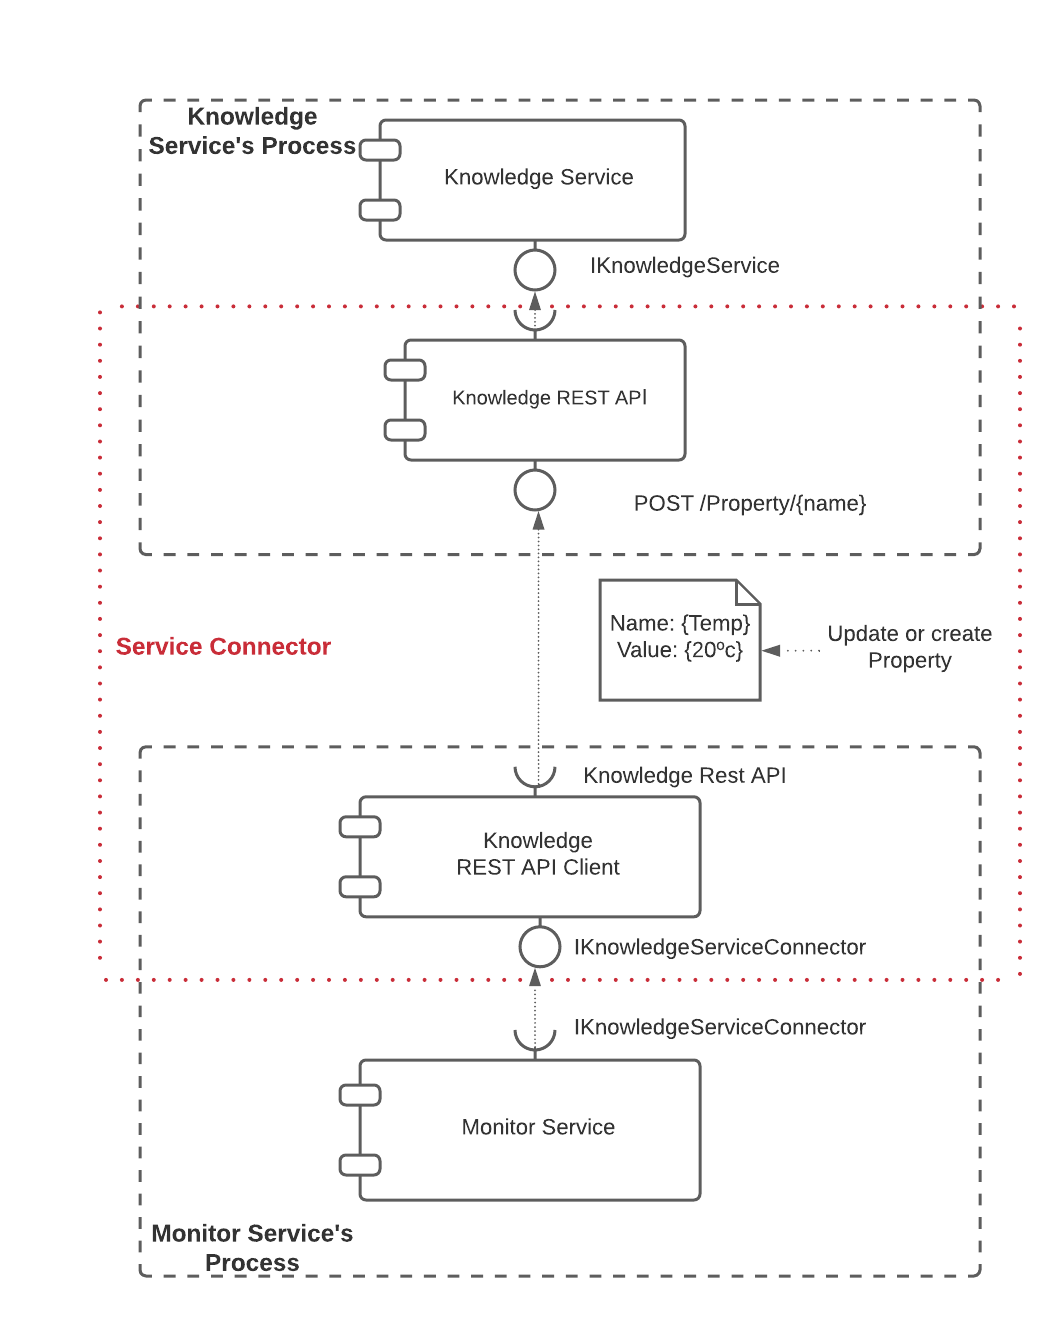
\includegraphics[scale=0.75]{02_arquitectura/images/Monitor-Knowledge-Connector}
  \caption{Diseño del conector usando implementación Cliente - Servidor}
  \label{fig:monitor-knowledge-connector}
\end{figure}

\pagebreak

\subsection{Open API}

\begin{wrapfigure}{r}{0.35\linewidth}
  % \vspace{15pt}
  
\includegraphics[scale=0.34]{02_arquitectura/images/openapi-logo}
  \centering
  % \vspace{15pt}
\end{wrapfigure}

OpenAPI\footnote{Open API specification: \url{https://spec.openapis.org/oas/latest.html}} es un lenguaje estándar para describir APIs implementadas sobre el protocolo HTTP. Es un \textit{domain specific language} que podemos utilizar para describir APIs de nuestras aplicaciones

Para el desarrollo de este trabajo, hemos optado por utilizar conectores basados en APIs REST. Nos permitía utilizar mecanismos ya presentes en los microservicios que queríamos desarrollar, y que fueran más homogéneos.
Para facilitar la compatibilidad de los microservicios, y facilitar el desarrollo de nuevos microservicios, hemos decidido usar la especificación OpenAPI.

La principal ventaja que nos ofrecía OpenAPI era la posibilidad de generar código a partir de la especificación. Permite generar código tanto del cliente como del servidor. De esta forma, podíamos implementar nuestra API genérica en un lenguaje . En este caso, se decidió utilizar conjuntamente el lenguaje C\# junto con el framework ASP.NET Core, para implementar los microservicios iniciales.

A partir de estos microservicios, podemos exportar la especificación de OpenAPI, haciendo uso de los endpoints, atributos y comentarios. Por ejemplo, en este endpoint del servicio de monitorización, vemos cómo obtiene una propiedad del servicio de conocimiento.

Podemos observar cómo el método está decorado con atributos que describen el tipo de respuesta que produce, según el código de respuesta HTTP. Estos comentarios se utilizan en la generación de la especificación para obtener mejor implementación

Después, haciendo uso de las librerías de generación de código de OpenAPI.


\chapter{Caso de estudio: Sistema de climatización}
\label{chap:caso_estudio}

Para verificar la arquitectura definida, decidimos implementar un pequeño sistema autoadaptativo. Se trata de un sistema de climatización, que gestiona la temperatura de una habitación. Para ello, dispondremos de un aire acondicionado, que calentará o enfriará la habitación según corresponda.

\section{Análisis}

El primer paso es capturar los requisitos del sistema a implementar. Cómo hemos comentado, queremos desarrollar un sistema de climatización. Este sistema regulará la temperatura de una habitación mediante el uso de un aparato de aire acondicionado.

El aparato de aire acondicionado ofrece tres modos de funcionamiento: un modo para calentar la estancia, otro para enfriarla, y un estado neutral (apagado). Además, lo hemos dotado con un termómetro interno que nos reporta la temperatura periódicamente.

Para poder climatizar la habitación, necesitamos que el usuario defina su temperatura objetivo: la temperatura de confort. Cambios en la temperatura deberán activar o desactivar el aparato para mantenerla.

Además, nos interesa evitar que el aire acondicionado se encienda y se apague constantemente cuando se alcance o sobrepase esta temperatura. Por ello, definimos unas temperaturas umbrales, tanto de frío como de calor, a partir de las cuales se encenderá el aparato.

\section{Diseño}

Del análisis anterior ya podemos deducir la existencia de dos componentes: un aparato de aire acondicionado (el sistema gestionado) y un termómetro (la sonda). Aparte de ellos, deberemos implementar la infraestructura necesaria para comunicarse con nuestro bucle MAPE-K: monitores, módulos de reglas y efectores que nos permitan interactuar con el sistema manejado.

Para describir el diseño usaremos la notación de sistemas autoadaptativos descrita en \cite{fonsEspecificacionSistemasAutoadaptativos2021}.

\subsection{Sondas:}

Para implementar el sistema, requerimos de las siguientes sondas:

\begin{longtable}{|r p{11.5cm}|}
    \hline
    \textbf{Sonda:} & \emph{thermometer}  \\
    \textbf{Descripción:} & Reporta la temperatura actual de la habitación (en ºc). \\
    \textbf{Monitor:} & \emph{Climatisation.Monitor} \\
    \textbf{Datos:} & \emph{temperature} \\
    \hline
    \textbf{Sonda:} & \emph{airconditioner-mode-changed-probe}  \\
    \textbf{Descripción:} & Reporta el modo de funcionamiento del aire acondicionado cuando este cambia. \\
    \textbf{Monitor:} & \emph{Climatisation.Monitor} \\
    \textbf{Datos:} & \emph{airconditioner-mode} \\
    \hline
    \textbf{Sonda:} & \emph{airconditioner-adaption-loop-registration}  \\
    \textbf{Descripción:} & Cuando arranca el servicio de aire acondicionado, registra la configuración inicial del sistema. \\
    \textbf{Monitor:} & \emph{Climatisation.Monitor} \\
    \textbf{Datos:} & \emph{airconditioner.is-deployed}, \emph{airconditioner-mode}, \emph{target-temperature}, \emph{cold-temperature-threshold}, \emph{hot-temperature-threshold} \\
    \hline

    \caption{Sondas del sistema de climatización.}
    \label{tab:climatisation-probes}
\end{longtable}

\subsection{Propiedades de adaptación:}

También podemos deducir cuáles son nuestras propiedades de adaptación:

\begin{longtable}{|r p{11.5cm}|}
    \hline
    \textbf{Propiedad:} & \emph{temperature}  \\
    \textbf{Descripción:} & Representa la temperatura actual de la habitación (en ºC).  \\
    \textbf{Tipo de dato:} & \emph{float} \\
    \hline
    \textbf{Propiedad:} & \emph{target-temperature}  \\
    \textbf{Descripción:} & La temperatura de confort definida por el usuario. El sistema deberá adaptarse para alcanzarla.  \\
    \textbf{Tipo de dato:} & \emph{float} \\
    \hline
    \textbf{Propiedad:} & \emph{cold-temperature-threshold}  \\
    \textbf{Descripción:} & La temperatura umbral de frío (en ºc). Si la temperatura baja por debajo de este umbral, deberá calentarse la habitación. \\
    \textbf{Tipo de dato:} & \emph{float} \\
    \hline
    \textbf{Propiedad:} & \emph{hot-temperature-threshold}  \\
    \textbf{Descripción:} & La temperatura umbral de calor (en ºc). Si la temperatura sube por encima de este umbral, deberá enfriarse la habitación. \\
    \textbf{Tipo de dato:} & \emph{float} \\
    \hline
    \textbf{Propiedad:} & \emph{airconditioner.is-deployed}  \\
    \textbf{Descripción:} & Indica si el servicio de aire acondicionado está desplegado y en funcionamiento.  \\
    \textbf{Tipo de dato:} & \emph{bool} \\
    \hline
    \textbf{Propiedad:} & \emph{airconditioner-mode}  \\
    \textbf{Descripción:} & Representa el modo de operación actual del aire acondicionado: \emph{Off} = 0, \emph{Cooling} = 1, \emph{Heating} = 2  \\
    \textbf{Tipo de dato:} & Enumerado \\
    \hline

  \caption{Propiedades de adaptación del sistema de climatización.}
  \label{tab:climatisation-adaption-properties}
\end{longtable}

\subsection{Monitores:}

Necesitaremos definir varios monitores para capturar los datos de las sondas. En algunos casos, para evitar falsos positivos, y que se lleve a cabo adaptaciones provocadas por errores de medición, deberemos filtrar estos datos.

Por ejemplo, en el monitor de las temperaturas, \emph{climatisation.monitor.temperature}. Como en el ejemplo trabajamos con un aire acondicionado ficticio, le hemos establecido un margen de error grande: Si la nueva medida de temperatura está a 5ºc de diferencia o más, y hay menos de un minuto de diferencia entre ellas; la descartaremos. De esta forma, evitamos que el aire acondicionado se active o desactive por un error de medición.

\begin{longtable}{|p{3.7cm} p{10.7cm}|}
    \hline

    \textbf{Monitor:} & \emph{climatisation.monitor.temperature}  \\
    \textbf{Descripción:} & Recibe los reportes de temperatura de los termómetros. También filtra estos datos para detectar casos donde se sospecha un error de lectura. \\
    \textbf{Afecta a propiedades de adaptación:} & \emph{temperature} \\
    \multirow{3}*{\textbf{Acciones:}}
        & \textbf{SI} |\emph{new-temperature} - \emph{temperature}| <= 5.0 \\
        & \textbf{O} request.DateTime - previousMeasurement.DateTime > 60s \\
        & \textbf{ACTUALIZA-KNOWLEDGE} \emph{temperature} = \emph{new-temperature} \\
    \hline

    \textbf{Monitor:} & \emph{climatisation.monitor.configuration}  \\
    \textbf{Descripción:} & Recibe la configuración del aire acondicionado y la registra en el \emph{knowledge}. \\
    \textbf{Afecta a propiedades de adaptación:} & \emph{airconditioner.is-deployed}, \emph{airconditioner-mode}, \emph{target-temperature}, \emph{cold-temperature-threshold}, \emph{hot-temperature-threshold} \\
    \multirow{2}*{\textbf{Acciones:}}
        & \textbf{SI} \emph{property} != \emph{new-value} \\
        & \textbf{ACTUALIZA-KNOWLEDGE} \emph{property} = \emph{new-value} \\
    \hline

  \caption{Monitores del bucle MAPE-K del sistema de climatización.}
  \label{tab:climatisation-monitors}
\end{longtable}

\subsection{Reglas de adaptación}

En base a cambios de la temperatura local, deberemos decidir si es necesario llevar a cabo una acción correctiva. Por ejemplo, que si la temperatura es inferior al umbral de temperatura fría, el aparato se enciende en modo calentador. Para ello, deberemos implementar un servicio de reglas (\emph{Climatisation.Rules.Service}). En él, incluiremos una serie de reglas que se disparen cuando cambie una de nuestras propiedades de adaptación. En este caso, la temperatura.

Como comentamos en el capitulo anterior, en nuestro ejemplo de bucle MAPE-K, nos limitamos a implementar las adaptaciones de tipo set-parameter. Por tanto, no tendremos reglas de despliegue o de binding.

En la tabla \ref{tab:adaption-rules-climatisation} definimos las cuatro reglas necesarias:

\begin{longtable}{|r p{12.8cm}|}
    \hline
    \textbf{Regla:} & \emph{EnableAirConditionerHeatingModeWhenColdTemperatureThresholdExceeded}  \\
    \textbf{Descripción:} & Activa el aire acondicionado en modo calefacción cuando la temperatura sea inferior al umbral de frío.  \\
    \textbf{Condición:} & \emph{airconditioner-mode} != \emph{Heating} \textbf{AND} \emph{temperature} <= \emph{cold-temperature-threshold}  \\
    \textbf{Cuerpo:}   &  \\
    & 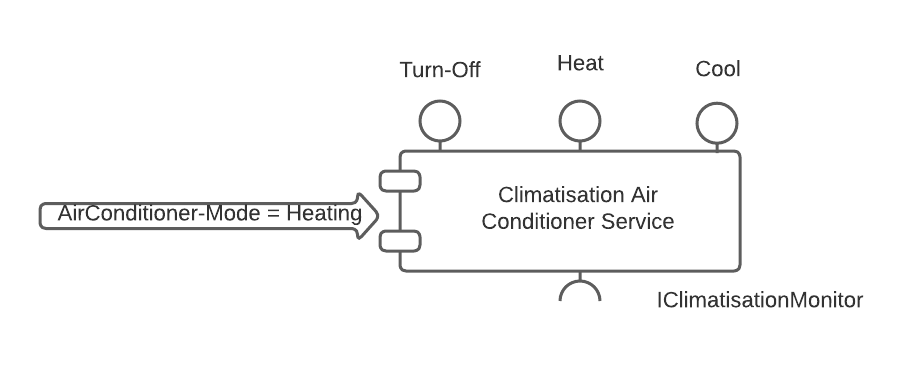
\includegraphics[scale=0.75]{04_caso-estudio/images/adaption-loop-rule-heat} \\
    \hline

    \textbf{Regla:} & \emph{DisableAirConditionerWhenHeatingModeEnabledAndTargetTemperatureAchieved}  \\
    \textbf{Descripción:} & Apaga el aire acondicionado cuando el modo calefacción está activo y se ha alcanzado la temperatura de confort.  \\
    \textbf{Condición:} & \emph{airconditioner-mode} == \emph{Heating} \textbf{AND} \emph{temperature} >= \emph{target-temperature}  \\
    \textbf{Cuerpo:} &  \\
    & 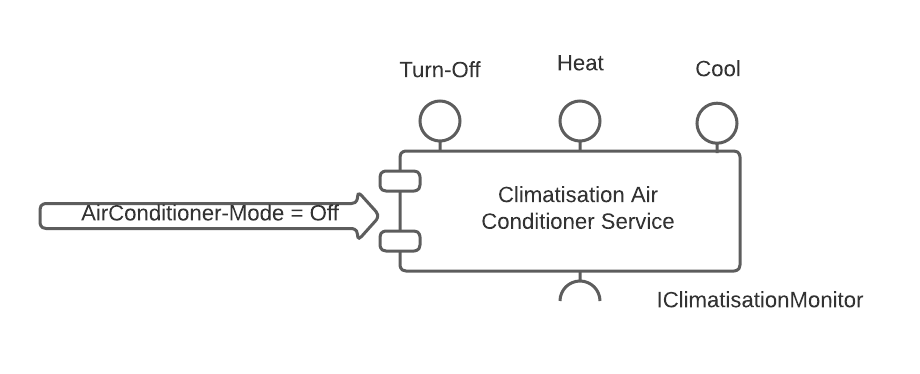
\includegraphics[scale=0.75]{04_caso-estudio/images/adaption-loop-rule-off} \\
    \hline

    \textbf{Regla:} & \emph{EnableAirConditionerCoolingModeWhenTemperatureThresholdExceeded}  \\
    \textbf{Descripción:} & Activa el aire acondicionado en modo enfriar cuando la temperatura sea superior al umbral de calor.  \\
    \textbf{Condición:} & \emph{airconditioner-mode} != \emph{Cooling} \textbf{AND} \emph{temperature} >= \emph{hot-temperature-threshold}  \\
    \textbf{Cuerpo:} &  \\
    & 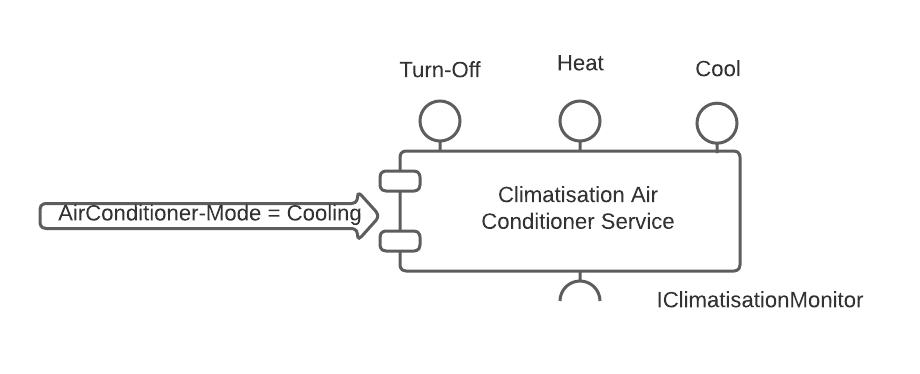
\includegraphics[scale=0.75]{04_caso-estudio/images/adaption-loop-rule-cooling} \\
    \hline

    \textbf{Regla:} & \emph{DisableAirConditionerWhenCoolingModeEnabledAndTargetTemperatureAchieved}  \\
    \textbf{Descripción:} & Apaga el aire acondicionado cuando el modo enfiar está activo y se ha alcanzado la temperatura de confort.  \\
    \textbf{Condición:} & \emph{airconditioner-mode} == \emph{Cooling} \textbf{AND} \emph{temperature} <= \emph{target-temperature}  \\
    \textbf{Cuerpo:} &  \\
    & 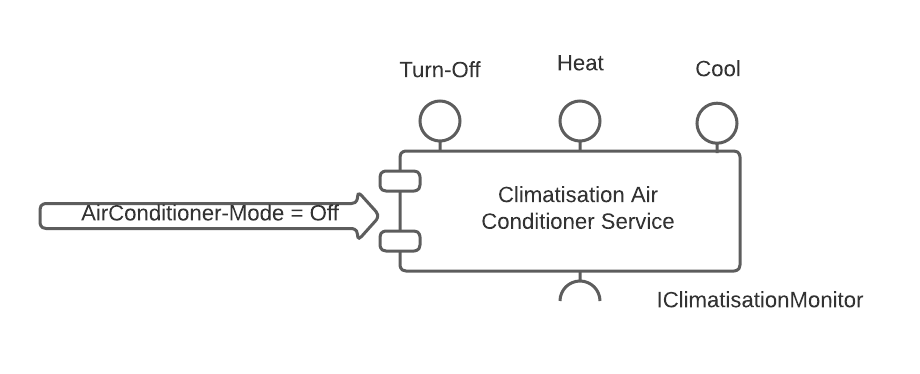
\includegraphics[scale=0.75]{04_caso-estudio/images/adaption-loop-rule-off} \\
    \hline

  \caption{Reglas de adaptación del sistema de climatización.}
  \label{tab:adaption-rules-climatisation}
\end{longtable}

\subsection{Efectores:}

Una vez se evaluén estas reglas, solicitamos un cambio en la configuración del sistema. El módulo de planificación comprobará contra el conocimiento y el estado actual del sistema cuáles de los cambios solicitados es necesario aplicar. Si por ejemplo la propiedad ya tiene el valor solicitado, no hará falta ejecutarla.

El modulo de ejecución recibirá la petición y se la redirigirá a los efectores del sistema de climatización. En este caso, requerimos de efectores que cambien el modo del aire acondicionado según corresponda.

\begin{table}[htb]
  \centering

  \begin{tabular}{|r p{11.5cm}|}
    \hline
    \textbf{Efector:} & \emph{airconditioner.heat}  \\
    \textbf{Descripción:} & Activa el modo calentar del aire acondicionado. \\
    \hline
    \textbf{Efector:} & \emph{airconditioner.cool}  \\
    \textbf{Descripción:} & Activa el modo enfriar del aire acondicionado. \\
    \hline
    \textbf{Efector:} & \emph{airconditioner.turn-off}  \\
    \textbf{Descripción:} & Apaga el aire acondicionado. \\
    \hline
  \end{tabular}

  \caption{Efectores del sistema de climatización.}
    \label{tab:climatisation-effectors}
\end{table}

Hecho esto, el sistema se adapta a a la nueva situación, y reportará una nueva temperatura en cuanto corresponda. La temperatura variará dependiendo de si está apagado o no.

\subsection{Configuración del sistema}

Requerimos entonces 4 servicios para implementar la solución: Servicio de aire acondicionado, monitor de climatización, el servicio de reglas y el servicio de efectores. Con ellos, podemos adaptarnos al bucle MAPE-K descrito en el capítulo %TODO: Capítulo.

\section{Implementación}

Para la implementación, hemos utilizado las mismas tecnologías que en los servicios del bucle MAPE-K: microservicios en ASP.NET Core, empaquetados en contenedores de Docker para facilitar su despliegue. Generamos los API Clients con OpenAPI y demás.

Como no disponemos de un aire acondicionado real, hemos optado por implementar uno ficticio. Cuando está apagado, la temperatura aumenta o disminuye según una configuración del fake. De esta forma, podemos simular los cambios de temperatura más rápido y ver si se aplican las adaptaciones pertinentes.

\subsection{Telemetría}

Un punto en el que queremos hacer hincapié es en la telemetría. Debido a que estamos tratando con un sistema distribuido es complicado conocer el estado del sistema en determinado momento. Especialmente en este caso, que participan más de diez servicios distintos.

Por defecto, solo contábamos con los \emph{logs} de consola, que mostramos en la figura \ref{fig:console-logs}. Aparecen en una única ventana intercalados los registros de todos los servicios. Aunque nos pueden resultar útil, es una aproximación ineficiente y según aumente la escala de peticiones simultáneamente se volverá más difícil de interpretar.

\begin{figure}[h]
  \centering
  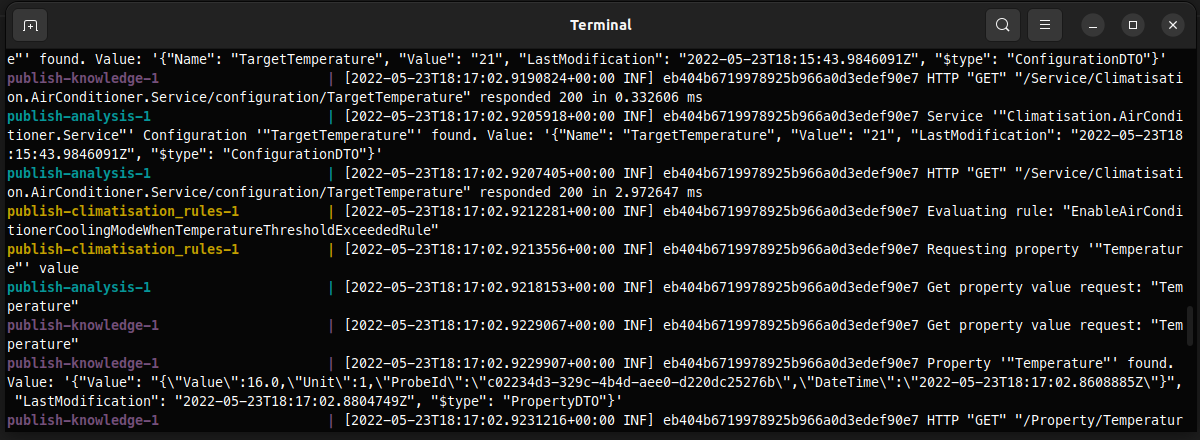
\includegraphics[scale=1.45]{04_caso-estudio/images/console-logs}
  \caption{Extracto de \emph{logs} de una ejecución habitual.}
  \label{fig:console-logs}
\end{figure}

Por ello, para que resultara más sencillo trabajar en la implementación de los servicios y diagnosticar qué ocurre con el sistema, decidimos implementar una solución de observabilidad. La observabilidad es \cite{parkerProblemDistributedTracing2020} y consta de tres partes distintas: %TODO CITA
\begin{itemize}
  \item \textbf{Logs}: A recording of an Event. Typically the record includes a timestamp indicating when the Event happened as well as other data that describes what happened, where it happened, etc. \cite{opentelemetryOpenTelemetryDocumentation2022} Provide extremely fine-grained detail on a given service, but have no built-in way to provide that detail in the context of a request. \cite{parkerProblemDistributedTracing2020}
  \item \textbf{Métricas}: Son agregados que nos permiten conocer el estado de las estancias de nuestros servicios. Records a data point, either raw measurements or predefined aggregation, as timeseries with Metadata. \cite{opentelemetryOpenTelemetryDocumentation2022}
  \item \textbf{Trazas distribuidas}: Tracks the progression of a single Request, called a Trace, as it is handled by Services that make up an Application. A Distributed Trace transverses process, network and security boundaries. \cite{opentelemetryOpenTelemetryDocumentation2022}  providing visibility into the operation of your microservice architecture. It allows you to gain critical insights into the performance and status of individual services as part of a chain of requests in a way that would be difficult or time-consuming to do otherwise. Distributed tracing gives you the ability to understand exactly what a particular, individual service is doing as part of the whole, enabling you to ask and answer questions about the performance of your services and your distributed system. \cite{parkerProblemDistributedTracing2020}
\end{itemize}

Para poder capturar todos estos elementos, optamos por usar el estándar OpenTelemetry. Se trata de una librería estándar utilizada para instrumentar el código de las aplicaciones. Distintas compañías del ámbito de la telemetría software ofrecen APIs que capturan el output de esta librería.

Gracias a él pudimos capturar la telemetría de la siguiente forma implementar usando tres servicios distintos:

\begin{figure}[h]
  \centering
  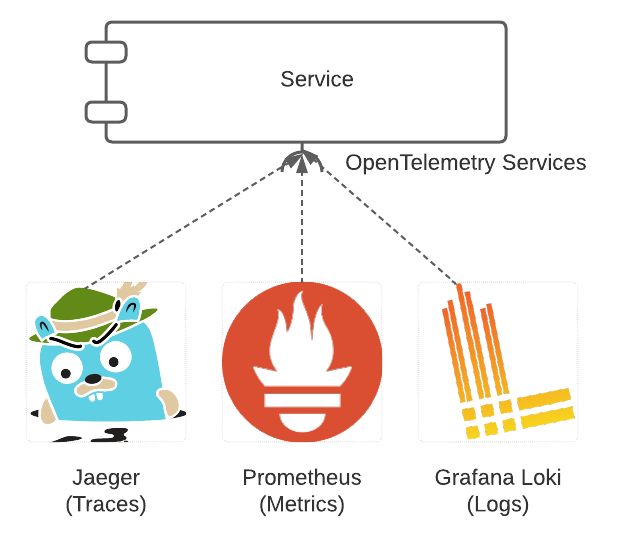
\includegraphics[scale=0.75]{04_caso-estudio/images/observability-telemetry-collection}
  \caption{Extracto de \emph{logs} de una ejecución habitual.}
  \label{fig:observability-telemetry-collection}
\end{figure}

\subsubsection{Loki: Logs}
Lo primero que queremos ver es cómo mejorar nuestra estrategia de logging. Lo ideal es añadir identificadores de correlación (el traceID), que nos permita rastrear a través de los distintos servicios una misma traza. Por ejemplo, podemos filtrar a partir de ella para ver todos los detalles de los servicios que intervinieron.

\subsubsection{Jaeger: Trazas distribuidas}

Gracias a las trazas distribuidas, podemos ver todas las actividades por las que pasó una petición. En nuestro caso, podemos ver por todos los estados por los que paso.

\subsubsection{Prometheus: Métricas}


\subsubsection{Grafana: Visualización}

Desarrollamos un panel de monitorización con Grafana. Esto nos permitía consultar en un solo lugar las métricas, los logs y las trazas.


%%%%%%%%%%%%%%%%%%%%%%%%%%%%%%%%%%%%%%%%%%%%%%%%%%%%%%%%%%%%%%%%%%%%%%%%%%%%%%%
%                                 CONCLUSIONS                                 %
%%%%%%%%%%%%%%%%%%%%%%%%%%%%%%%%%%%%%%%%%%%%%%%%%%%%%%%%%%%%%%%%%%%%%%%%%%%%%%%

\chapter{Conclusions}

????? ????????????? ????????????? ????????????? ????????????? ?????????????

%%%%%%%%%%%%%%%%%%%%%%%%%%%%%%%%%%%%%%%%%%%%%%%%%%%%%%%%%%%%%%%%%%%%%%%%%%%%%%%
%                                BIBLIOGRAFIA                                 %
%%%%%%%%%%%%%%%%%%%%%%%%%%%%%%%%%%%%%%%%%%%%%%%%%%%%%%%%%%%%%%%%%%%%%%%%%%%%%%%

\bibliography{bibliography}

\cleardoublepage

%%%%%%%%%%%%%%%%%%%%%%%%%%%%%%%%%%%%%%%%%%%%%%%%%%%%%%%%%%%%%%%%%%%%%%%%%%%%%%%
%                           APÈNDIXS  (Si n'hi ha!)                           %
%%%%%%%%%%%%%%%%%%%%%%%%%%%%%%%%%%%%%%%%%%%%%%%%%%%%%%%%%%%%%%%%%%%%%%%%%%%%%%%

\APPENDIX

%%%%%%%%%%%%%%%%%%%%%%%%%%%%%%%%%%%%%%%%%%%%%%%%%%%%%%%%%%%%%%%%%%%%%%%%%%%%%%%
%                         LA CONFIGURACIO DEL SISTEMA                         %
%%%%%%%%%%%%%%%%%%%%%%%%%%%%%%%%%%%%%%%%%%%%%%%%%%%%%%%%%%%%%%%%%%%%%%%%%%%%%%%

\chapter{Configuració del sistema}

????? ????????????? ????????????? ????????????? ????????????? ?????????????

\section{Fase d'inicialització}

????? ????????????? ????????????? ????????????? ????????????? ?????????????

\section{Identificació de dispositius}

????? ????????????? ????????????? ????????????? ????????????? ?????????????

%%%%%%%%%%%%%%%%%%%%%%%%%%%%%%%%%%%%%%%%%%%%%%%%%%%%%%%%%%%%%%%%%%%%%%%%%%%%%%%
%                               ALTRES  APÈNDIXS                              %
%%%%%%%%%%%%%%%%%%%%%%%%%%%%%%%%%%%%%%%%%%%%%%%%%%%%%%%%%%%%%%%%%%%%%%%%%%%%%%%


\chapter{??? ???????????? ????}

????? ????????????? ????????????? ????????????? ????????????? ?????????????



%%%%%%%%%%%%%%%%%%%%%%%%%%%%%%%%%%%%%%%%%%%%%%%%%%%%%%%%%%%%%%%%%%%%%%%%%%%%%%%
%                              FI DEL DOCUMENT                                %
%%%%%%%%%%%%%%%%%%%%%%%%%%%%%%%%%%%%%%%%%%%%%%%%%%%%%%%%%%%%%%%%%%%%%%%%%%%%%%%

\end{document}
